\documentclass[Preamble]{subfiles}
\begin{document}

\chapter{Prototype: School DNS}
A school want to use a DNS server to filter certain internet sites from students and also have the opportunity to get a faster response from the name server. 

\section{Solution}
To achieve the school's request, a BIND server could be set up. BIND is a open source implementation of the DNS protocols and is the most used DNS server software. One of the advantages with BIND, is that it supports both Windows, Mac and Linux. BIND acts like a caching server, where it stores answers to name queries and this results in reduced time of future queries to the same server.

When a requested hostname needs to be looked up, the local cache is the first place to be checked. If the hostname is not found there, the next DNS server is asked. This might be your ISP or even a server on a "higher" level. It is also possible via BIND to forward your requests to a public DNS, meaning the server will be asked, if no other server before that (e.g. your ISP's DNS) have the hostname in it's cache. 

\begin{figure}[hbtp]
\centering
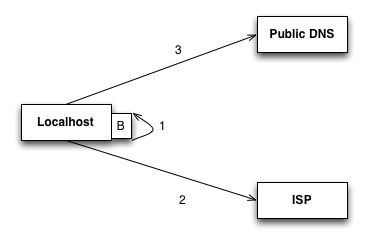
\includegraphics[scale=0.5]{../../Protoypes/DNS/ForwardingDiagram.jpg}
\caption{System overview}
\end{figure}


\subsection{Setup BIND Server}
To install a BIND server on Linux type in "sudo apt-get install bind[9]". This will install version 9 of the BIND server software. To check if installation if succesfull type "named -v" and if it is successfull, it will show "BIND 9.8.1-P1". For testing purpose, "dnsutils" have been used - and this can be used to see Query time for the DNS lookup with the commannd "dig -x [IP-address]"

\subsection{Forward to public DNS}
If the school whats to forward their requests to a public DNS, e.g. OpenDNS, they have to do a bit of research on finding the optimal solution for them. There is a lot of public DNS servers, where some servers are good at filtering bad hostnames, but are in the same time not always the fastest. In this section tests are made to find the fastest response time.

To find an optimal solution, Google's Test Bench (GTB) have been used. In this case GTB looked up around 4500 servers and tested them all to find the fastest server in average.

\begin{figure}[hbtp]
\centering
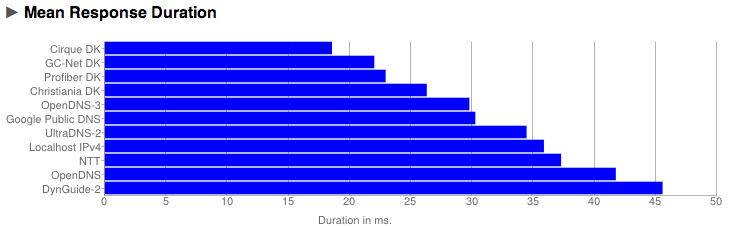
\includegraphics[scale=0.5]{Figurer/NamebenchTest.png}
\caption{Output from Google Test Bench test}
\end{figure}

The test shows, that Cirque DK have the lowest mean response time with 18ms, and the default   DNS have a mean response time on 36ms. One of the more popular public DNS is openDNS, which is a little faster than the default DNS with 29ms. To test if one of the public DNS is faster, a manual test with dig -x have been made with 5 different internet sites and their given response time. 

To test the given servers, the file located at /etc/bind/named have to be edited with the adress of the DNS server it shall forward to. 

\begin{center}
  \begin{tabular}{ l | c  | r}
    \multicolumn{3}{c}{Forwarding - Cirquie.DK}  \\
	\hline Site & First test (ms) & Second test (ms) \\     
    \hline
    Ubuntu.com & 391 & 381  \\ \hline
    Bt.dk & 356 & 906  \\ \hline
	Iha.dk & 375 & 240 \\ \hline
	Facebook.com & 354 &	207 \\ \hline
	Wikipedia.org & 375 & 442 \\ \hline
  \end{tabular}
\end{center}

\begin{center}
  \begin{tabular}{ l | c  | r}
    \multicolumn{3}{c}{Forwarding - OpenDNS}  \\
	\hline Site & First test (ms) & Second test (ms) \\     
    \hline
    Ubuntu.com & 355 & 352  \\ \hline
    Bt.dk & 792 & 436  \\ \hline
	Iha.dk & 334 & 117 \\ \hline
	Facebook.com & 184 & 279 \\ \hline
	Wikipedia.org & 153 & 115 \\ \hline
  \end{tabular}
\end{center}

It is hard to make a final conclusion based on our test, since the response times are unstable (e.g. Cirquie.DK with a response time on 356ms on Bt.dk in the first test, and 906ms in the second test and both test was under the same conditions), which is why Google Test Bench is a good tool to use. However, we can conclude that even if you forward to the one tested to be the fastest public DNS, you cannot be sure it is the fastest every single time, since it might be busy.

\subsection{Filtering}
A DNS server can also be used as a simple filter, in the way of not providing the IP for harmful or illegal hostnames. Some public DNS servers have this filter build-in, which means you in a simple way can archive a bit of security.

In the same way, it is also possible to block specific hostnames with BIND, which can be useful if you want your filter to be more specialized. This can be useful if a school wants to block for e.g. Facebook or Ekstrabladet.dk.

The problem about the filter is if the users look up the IP directly. In that case, the DNS server will not be used and the filter will therefore not be used either and other methods have to be used.

\subsection{Discussion}
There is a lot of ways of finding a solution for the school. To retrieve the caching functionality, BIND is simple and easy to set up and use. If wanted, it can furthermore be specialized in the way of setting up a filter or forwarding requests to a public DNS server.  

BIND is a simple solution, but if better security or caching is wanted, a custom solution is needed. However, for a small school this might not be needed, and therefore BIND would be the suggested choice.

\end{document} 